\section{Vježba 3: Houghova transformacija}

\subsection{Opis vježbe}
Potrebno je pomoću, prethodno kalibrirane, web kamere uslikati objekt
kvadratnog oblika koji je postavljen na milimetarskom papiru na stolu.
Primjenom Houghove transformacije (HT) treba odrediti parametre \(\rho
\) i \( \theta \)najdominantnijeg pravca, koji odgovara jednom od rubova objekta
na slici. Pod najdominantnijim pravcem podrazumijeva se pravac kojem
pripada najveći broj 'glasova' u akumulacijskoj ravnini. Implementacija
HT u biblioteci OpenCV vraća popis detektiranih pravaca koji su
razvrstani prema broju 'glasova' počevši od najdominantnijeg. Primjenom
odgovarajuće transformacije, odrediti \(\rho i \theta \)tog pravca u
koordinatnom sustavu milimetarskog papira. Provjeriti koliko je
odstupanje dobivenog pravca od stvarnog (odgovarajućeg) ruba objekta.

\subsection{Kalibracija kamere}
Cijenovna prihvatljivosti web kamera ima svoju negativnu stranu, a to je
značajna distorzija. Postoji radijalni efekt (\textit{fisheye}) i
tangencijalna distorzija (leće kamere nisu u savršeno paralelene s
ravninom slikanja). Zato kalibracijom kamere možemo rješiti te
nedostatke. Isto tako kalibracijom možemo odrediti vezu između piksela i
milimetara.

Za kalibraciju smo koristili program koji se kompajlira prilikom
kompajliranja OpenCV biblioteke. Pomoću njega smo dobili koeficiente
distorzije i matricu kamere. Te podatke program dobije računanjem
jednostavnih geometrijskih jednadžbi nad primjerom crno bijele šahovske ploče.

\begin{figure}[h]
\centering
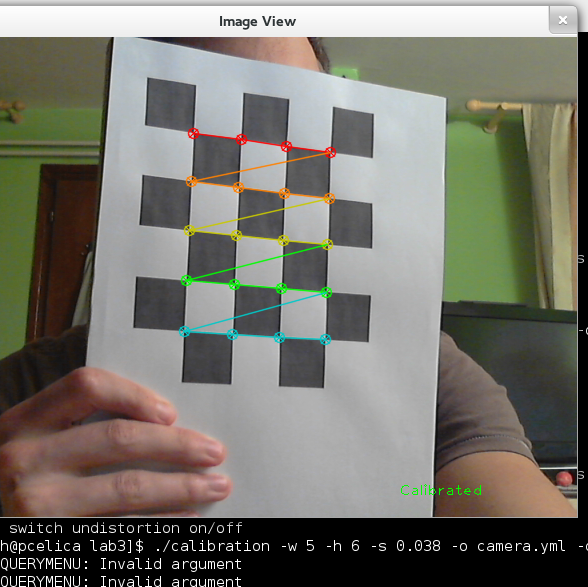
\includegraphics[scale=0.37]{images/lab3-01-calib.png}
\caption{Kalibracija kamere}
\label{fig:lab3-01-calib}
\end{figure}

\newpage
\subsection{Objašnjenje programa}

\subsubsection{Kontrola programa}

Prilikom pokretanja programa iz komandne linije potrebno je 
predati programu putanju do slike (argv[1]) ako nad njom želimo provesit
HT ili možemo uzeti sliku putem kamere.
\\
\begin{lstlisting}[language=C,caption={Kontrola programa tipkovnicom}]
while (1){
    char c = waitKey(10);
    switch(c) {
            case 'c':
                initCamera ();
                break;
            case 'h':
                if (!imageTaken) {
                    if (pointSelected) {
                        cannyEdge (loadedImg, ssBox);
                        cout << "Points?!1\n";
                    }
                    setMouseCallback (imageName, getPoints, 0);
                    cout << "No data from camera. Using argv[1] or \ default image\n";
                }
                else { 
                cannyEdge (ssImg, ssBox);
                }
                break;
            case 'H':
                callHoughTransform ();
                destroyWindow ("snapshot");
                break;
\end{lstlisting}

\begin{itemize}
    \item Pokrenut kameru pritiskom na ``c''
    \item Uslikati objekt na milimetarskom papiru s ``i''
    \item Označiti (klikom) četiri ugla milimetarskog papira
    \item Ugasiti kameru pritsikom na ``C''
    \item Pokrenuti filtiranje slike pritiskom na ``h''
    \item Pozvati houghovu transformaciju pritiskom na ``H''
\end{itemize}


\subsubsection{Houghova transformacija}
Detektiranje linija i određivanje  \(\rho \) i \( \theta \) u
koordinatnom sustavu milimetarskog papira je implementirano u funkciji
\textit{callHoughTransform()}.

\begin{lstlisting}[language=C,caption={Racunanje parametra ro i theta}]
int callHoughTransform ()
{
    /*
     * Find lines in edge point image using Hough Transform
     * HT is operating in polar coordinte system so our lines are
     * represented with: 
     * rho - vector from origin of c.s to line (perpendicular to line) 
     * theta - angle form positive x axis to rho (range -90-90)
     */
    vector<Vec2f> lines;
    HoughLines (cannyOut, lines, 1, CV_PI/180, 100, 0, 0);
    // cout << "Lines = " << Mat( lines ) << endl;
    if (lines.empty()) {
        cout << "HT didn't find lines, run edge with more details\n";
        return -1;
    }
    float rho, rhoRoi, theta;
    rhoRoi = lines[0][0];
    theta = lines[0][1];
    // Computes rho in image c.s.
    rho = rhoRoi + pt1.x * cos(theta) + pt1.y * sin(theta);
    // Read calibration parameters
    FileStorage fs ("../lab3/calib/cam-c270.xml", FileStorage::READ);
    // Intrinsics/projection matrix with fx,fy,u,v intrinsics camera
    // parameters for unit conversion
    Mat intrinsics (3, 3, CV_32F); 
    fs ["camera_matrix"] >> intrinsics; 
    // Distortion matrix with k1,k2,p1,p2,k3 distortion coefficients
    // for correcting cameras radial and tangential distortion
    Mat distortion (5, 1, CV_32F);
    fs ["distortion_coefficients"] >> distortion; 
    // Dimension's of graph paper in mm
    vector<Point3f> objectPoints (4);
    objectPoints[0] = Point3f (0, 0, 0);
    objectPoints[1] = Point3f (0, 265, 0);
    objectPoints[2] = Point3f (170, 0, 0);
    objectPoints[3] = Point3f (170, 265, 0);
    // Rotation vector output from solvePnP
    Mat rvec (1, 3, CV_32F);
    // Translation vetor - descrabise position of object c.s.     
    // in regards to camera c.s
    Mat tvec (1, 3, CV_32F);
    // Estimate object position from 3D-2D point correspondences.
    solvePnP (Mat (objectPoints), Mat (imagePoints), intrinsics,
            distortion, rvec, tvec, false);
    // Rotation matrix - describes orientation of object c.s. 
    // in regards to camera c.s
    Mat R (3, 3, CV_32F);
    // Converts rotation vector to rotation matrix
    Rodrigues (rvec, R);
    //cout << "R = " << R <<  endl;
    // A matrix store unit converted rotation matrix
    Mat A (3, 3, CV_32F);
    A = intrinsics * R; 
    // B vector stores crorrected translation vector
    Mat B (3, 1, CV_32F);
    B = intrinsics * tvec;
    double lambdaX, lambdaY, lambdaRo, rhoCrtano, thetaCrtano;
    lambdaX = A.at<double>(0,0) * cos(theta) + A.at<double>(1,0) *
        sin(theta) - rho * (A.at<double>(2,0));
    lambdaY = A.at<double>(0,1) * cos(theta) + A.at<double>(1,1) *
        sin(theta) - rho * (A.at<double>(2,1));
    lambdaRo = rho * (B.at<double>(2)) - B.at<double>(0) * 
        cos(theta) - B.at<double>(1) * sin(theta); 
    thetaCrtano = atan2 (lambdaY, lambdaX);
    rhoCrtano = lambdaRo / sqrt (lambdaX * lambdaX + lambdaY * lambdaY);
    cout << "Theta = " << thetaCrtano*180/CV_PI "degres" << endl;
    cout << "Rho = " << rhoCrtano << "mm" << endl;
    return 0;
}
\end{lstlisting}

\newpage
\begin{figure}
\centering
\begin{minipage}{.5\textwidth}
  \centering
  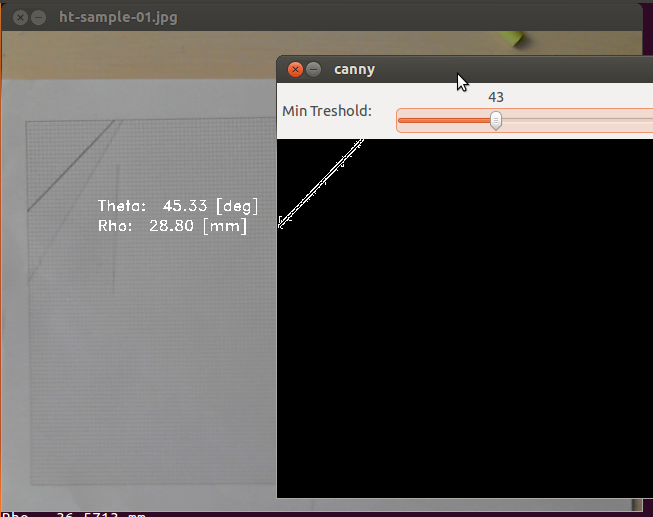
\includegraphics[width=.9\linewidth]{images/lab3-sample-01.png}
  \caption{A figure}
  \label{fig:test1}
\end{minipage}%
\begin{minipage}{.5\textwidth}
  \centering
  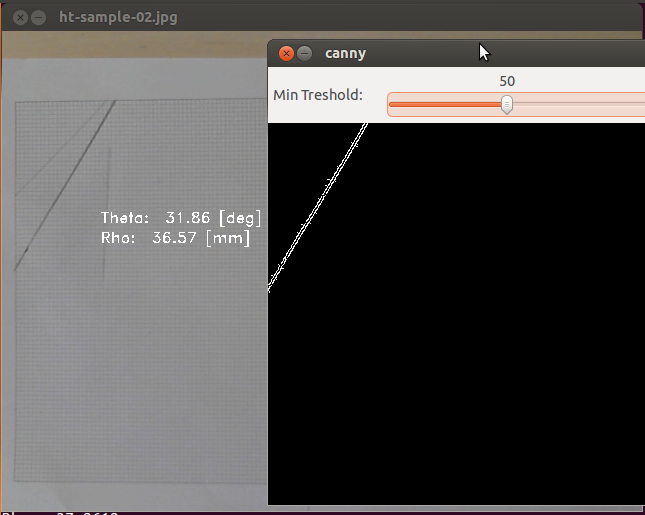
\includegraphics[width=.9\linewidth]{images/lab3-sample-02.png}
  \caption{Another figure}
  \label{fig:test2}
\end{minipage}
\end{figure}

\begin{figure}[h]
\centering
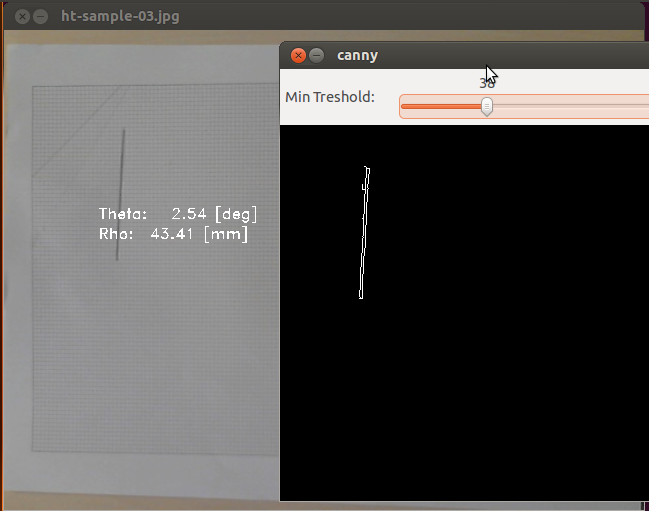
\includegraphics[scale=0.32]{images/lab3-sample-03.png}
\caption{Houghova transformacija}
\label{fig:lab3-sample-03}
\end{figure}

\subsection{Rezultati}

\begin{center}
\centering
\begin{tabular}
{ l || c | c | p{1.6 cm} | p{1.6 cm}  }
{uzorak}  & {\(\theta\) $[mm]$ } & {\(\rho \) $[mm]$} & {izmjerena \(\theta\) $[mm]$} & {izmjeren \(\rho\) $[mm]$} \\ \hline
ht-sample-01 & 45.33 & 28.80 & 45 & 30 \\ \hline
ht-sample-02 & 31.86 & 36.57 & 32 & 39 \\ \hline
ht-sample-03 & 2.54 & 43.41 & 3 & 44 \\ 
\end{tabular}
\end{center}

\newpage
\subsection{Zaključak}

